\label{sec:evaluation}

\section{Overview}
A usability evaluation was carried out on the deployed version of \emph{rmt} which had 11 hosts in the yellow tower running the client-side software stack, with the Pi Master running the server-side stack, described in section \ref{sec:arch}.

The user was given a task sheet, attached in appendix \ref{app:tasksheet}, and asked to carry out the tasks under observation.
Notes were taken regarding each user's session, which typically lasted less than five minutes.
Once the tasks were completed the user was asked to complete a questionnaire hosted on Google docs, a screenshot of which can be seen in appendix \ref{app:questionnaire}.

Some feedback from the demonstration is also considered.

\section{Setup}

As mentioned above, there were 11 hosts in the yellow tower, each of which were running the full client-side software stack with the exception of 192.168.1.22, which was not and appeared in the dead (grey) state.
Two hosts were removed from the tower so that the user could see the ``Unassigned Hosts'' section in the add page, and so that they had hosts to add to the tower in the tasks.


\section{Task sheet}

Under supervision, users were asked to complete a series of tasks as previously mentioned.
Every task was completed successfully by every user except tasks 6 and 7.
These tasks asked the user to identify which hosts were running containers and which were not, identifying one example in each case.

The two users who failed one or both of these tasks described the hosts in a non-``fine'' state as not running containers.
This represents a disparity between user expectation and system expectation.
The system expects the user to understand that the changing state represents whether the host is running or not, and with the users not being familiar with PiCloud or with containers, it is evident that the heartbeat, in its current state, is not immediately intuitive.

After the exercise they were given feedback and upon explanation, the users fully understood.
The disparity between user and system expectations could perhaps be linked to a lack of understanding of the PiCloud and of containers, but it should also be noted that there is a failing in the user interface for users unfamiliar with the project.

This is not necessarily a failing of the project in general however as the general public are not expected to use this system and fully understand it at first glance.
Similar systems such as the aforementioned Shipyard and DockerUI would possibly face similar problems if given to people with little understanding of containers.

Another feature expected by four of the seven users to participate in the evaluation was ``click-and-drag'' moving of hosts to other towers.
In the second task the user is asked to add a host to the red tower, and to accomplish this task these four users clicked on a host in the yellow tower and tried to drag it to the red tower, as shown in figure \ref{fig:clickanddrag}

\begin{figure}[t]
	\centering
	\setlength\fboxsep{0pt}
	\setlength\fboxrule{0.5pt}
	\fbox{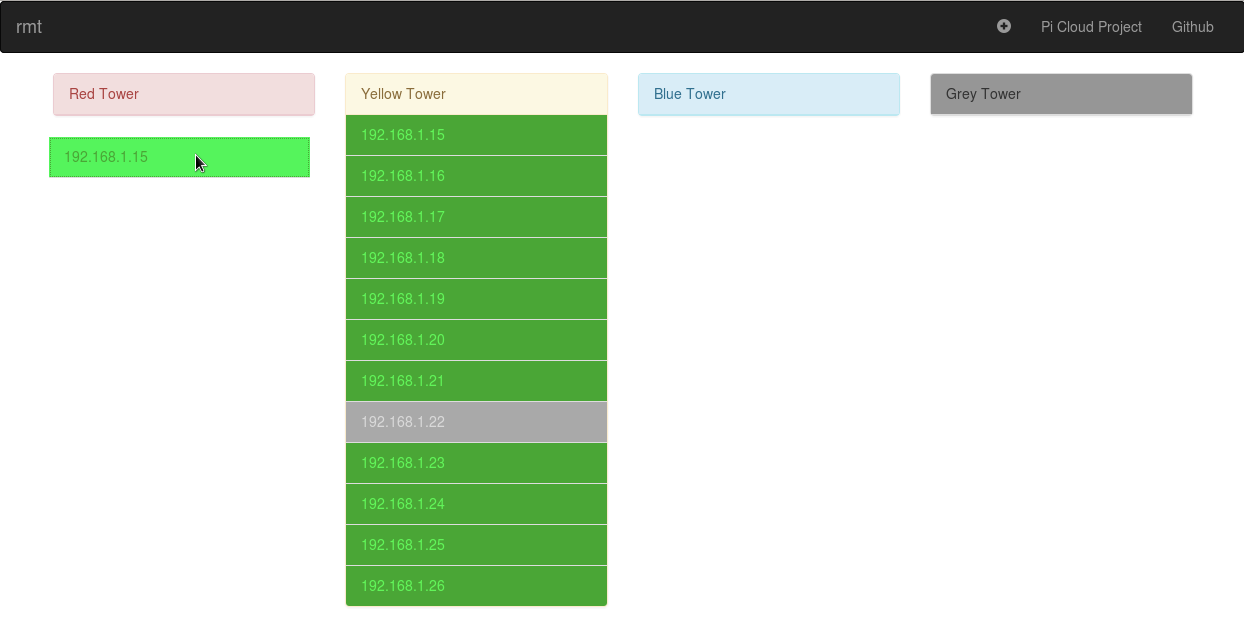
\includegraphics[width=0.8\textwidth]{clickAndDrag}}
	\caption{Recreation of a user attempting to click-and-drag a host to a tower}
	\label{fig:clickanddrag}
\end{figure}

Given that so many users tried this, a discussion was brought up with stakeholders in the project and they stated that this would not be a useful operation as they rarely move the hosts between the physical towers, being able to do this in \emph{rmt} is therefore not a requirement and not planned as future work.

Two of the participants tried to click on a tower to add a host.
This was interesting as with the harsher colour scheme of the hosts and with the hosts changing to a slightly lighter colour when the mouse moves over them it was thought this would be clear to the user that those elements were clickable, while static elements, such as the tower headings, would clearly not be clickable.
It is not an unreasonable feature however, and this could help speed up the adding process as the tower would already be selected and the user would simply have to enter the host address.

\section{Questionnaire Feedback}

Raw questionnaire feedback data can be seen in appendix \ref{app:feedback}.

Users were asked to fill out this questionnaire and told explicitly that they did not have to fill it out if they did not want to and that they could fill out as much, or as little, as they wanted to.
Luckily for the evaluation, almost every question was answered by every user.

Some of this feedback is excellent and gives the project great features for future work and this was the reason for having the questionnaire focused on qualitative feedback over quantitative feedback.

The first user stated that during the evaluation they would have been more aware of the system's purpose if they had been given an overview beforehand and this was admittedly a mistake that was not repeated after this.

In terms of usefulness the most important questions were the final two, both of which are answered well in the majority of cases.
Four of the seven participants indicated a need for greater depth of information on the home page, which ties in with the ``at-a-glance'' requirement of the software.
In its current state, the participants correctly noted that the home page has very little information regarding the containers of each host and that this information would be better suited to the home page, or at least the number of containers shown would be useful.
This is up to the stakeholders of the PiCloud project to decide, however monitoring of containers on the home page would be useful and mean that users would not have to search for a container by clicking each and every individual host since this does not scale well.

\section{Demonstration Feedback}

Currently, to add multiple hosts, the user has to add each one individually and this is not scalable.
Before the demonstration it was not known that each tower had its own subnet, so the tower could have been automatically assigned based on this which removes the need for the user to specify it.
Without having to specify the tower, adding hosts can be done automatically based on whether or not it is running the client-side software stack.
